\documentclass[UTF8]{ctexart}
\usepackage{graphicx}
\usepackage{listings}

\title{实验六报告}
\author{唐灵\\519030910052\\F1903002}
\date{\today}
\begin{document}
    \maketitle
    \begin{abstract}
        这是电工导c课程的第五次实验
    \end{abstract}
    \section{实验概览}
        本次实验情况特殊,实验开始的时候,我在docker中连 searchFiles.py 都没有办法运行,关于环境的问题已经严重影响了我之前两次的作业!

        无法每次都借同学的电脑,所以最终选择逃离java,选择whoosh作为文本检索的框架进行进一步的实验。
        
        话说回来,本次实验使用Flask,结合前面学习的HTML,中文分词等知识点,根据上次实验爬取的网页,建立一个简单的搜索引擎。

        在这次实验中,我将用whoosh取代Lucene,并重写建立索引,写入索引,以及搜索模块三个模块的内容。这也是对上一次无法进行实验的弥补。
        
        当然,也完成了本次实验的关键部分,也就是将使用flask,完成基本的网页构建。
    \section{实验环境}
        本次作业文本检索部分使用了whoosh,其他部分和课程要求内容完全一致,在本地环境中使用anaconda3完成实验,
        python的版本为3.8.5,具体环境环境如下:      
    \begin{figure}[ht]
        \centering
        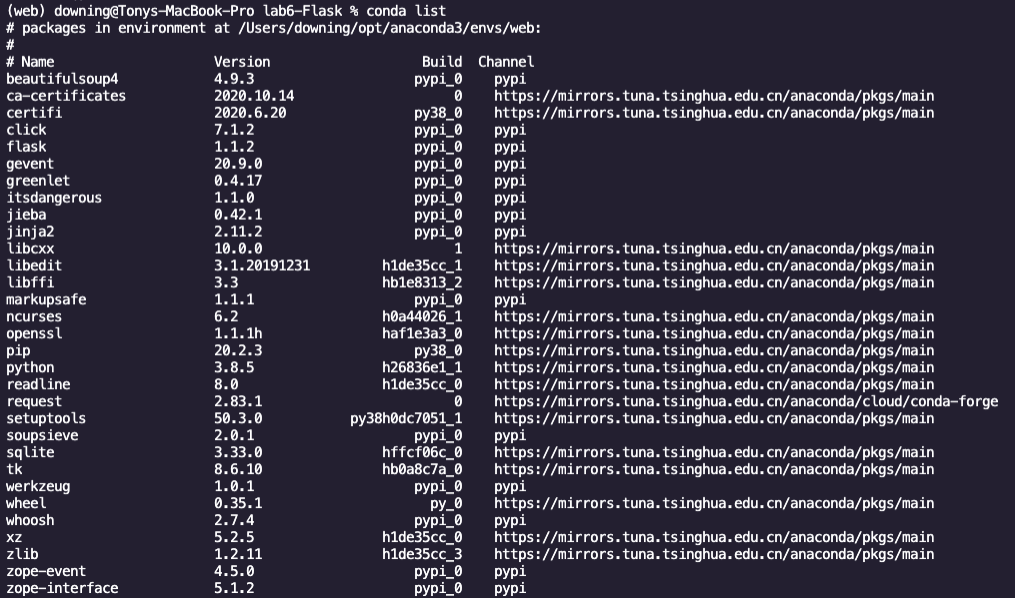
\includegraphics[scale=0.33]{img/env.png}
        \caption{实验运行环境}
    \end{figure} 
    \section{练习解决思路}
        \subsection{总体思路}
            总体的实现思路大致可以描述如下:
            \begin{enumerate}
                \item 服务器初始化根目录为搜索页面,通过 search.html 渲染模版。
                \item 程序猿从浏览器发起搜索,通过搜索页面向服务器发送请求,通过重定向到结果页面(由于页面设置,结果页面本身也是搜索页面),
                请求中后缀有"keyword"参数。
                \item 服务器通过获得keyword参数,再将keyword传入到search()函数,并返回搜索结果,这个函数来自于搜索模块,这个模块会对之前创建的索引进行搜索
                ,并返回所有的搜索结果,这个结果足够覆盖结果页面中我们用到的所有信息,并且已经进行过高亮处理。
                \item 将返回的搜索结果作为参数传入进网页模版 result.html 进行渲染,得到我们的搜索结果,再传回给浏览器。
            \end{enumerate}

        \subsection{请求表单}
            请求表单具有发送带有参数的请求的功能,写法如下图一般质朴无华:
            \begin{figure}[ht]
                \centering
                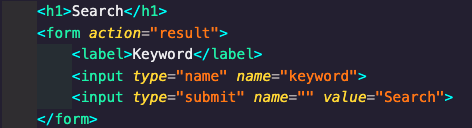
\includegraphics[scale=0.6]{img/form.png}
                \caption{表单}
            \end{figure}
        \subsection{搜索模块的实现}
            搜索模块的实现主要依赖于Whoosh的各种类,跟Lucene的逻辑非常相似,并且jieba有专门针对于Whoosh的接口,所以
            对于中文分词也不必过多的担心,直接在建立索引的时候对于content字段的分析器采用jieba的ChineseAnalyzer即可,这样就省掉了大量的麻烦。

            对于whoosh,必须要求所有的存入的字符都采用unicode编码,这使得中文的编码问题也不再是问题。

            针对于高亮搜索,我们希望搜索结果返回周围的少部分文字,并且希望关键字被一对合适的html标签包裹,
            这需要我们做进一步的定制:
            \begin{figure}[ht]
                \centering
                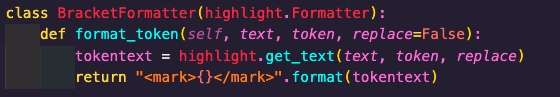
\includegraphics[scale=0.6]{img/highlight.png}
                \caption{高亮显示设定(包裹标签定制)}
            \end{figure}

            最后值得一提的是,Whoosh搜索器返回的结果并非是python内置类型,如果直接传入到模版中进行迭代会出现问题,所以我们在过程中对这些搜索结果进行转化。

            最终返回的是一个列表,列表元素是每一个搜索结果,匹配程度越高排,序号越低。
            
            一个搜索结果由字典表达,字典中包含我们希望返回的信息:
            
            \begin{lstlisting}
                {
                    'title':'****',
                    'abstract':'****',
                    'url':'****'
                }
            \end{lstlisting}

        \subsection{网页模版的实现}
            主要关于结果页的网页模版:

            传入关键字和搜索结果两个参数,利用过滤器,得到第一行搜索提示,即返回这样的语句:告诉程序猿关于这个关键字的搜索结果我们找到了多少条?
            \begin{figure}[ht]
                \centering
                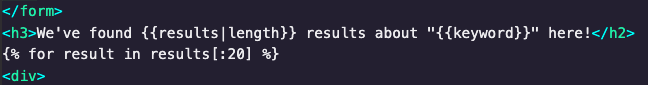
\includegraphics[scale=0.5]{img/tell.png}
                \caption{提示语句的写法}
            \end{figure}

            从上图也可以看出我们通过for循环对于我们的搜索结果进行打印。

            最后提一个东西,我们的传入的高亮字段也就是“abstract”,本身的关键字就已经被html标签包裹,但是开始的时候直接打印,在网页端只能够看到
            纯字符串,经查资料得到,这个设计是基于安全考虑,这里应该使用一个过滤器“safe”,来使得html标签能够被正确识别:
            \begin{figure}[ht]
                \centering
                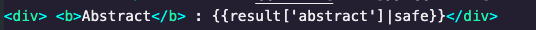
\includegraphics[scale=0.6]{img/hi.png}
                \caption{高亮语句导入}
            \end{figure}
    \section{代码运行结果}
        我们最终网页支持单字段和多字段搜索,这都是由自带的分析器进行完成,又少操心了,这里来显示一些搜索结果。

        \begin{figure}[ht]
            \centering
            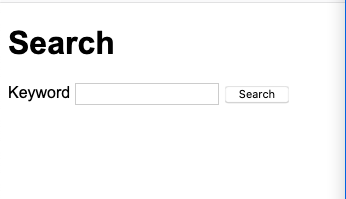
\includegraphics[scale=0.4]{img/search.png}
            \caption{初始化页面}
        \end{figure}

        \begin{figure}[ht]
            \centering
            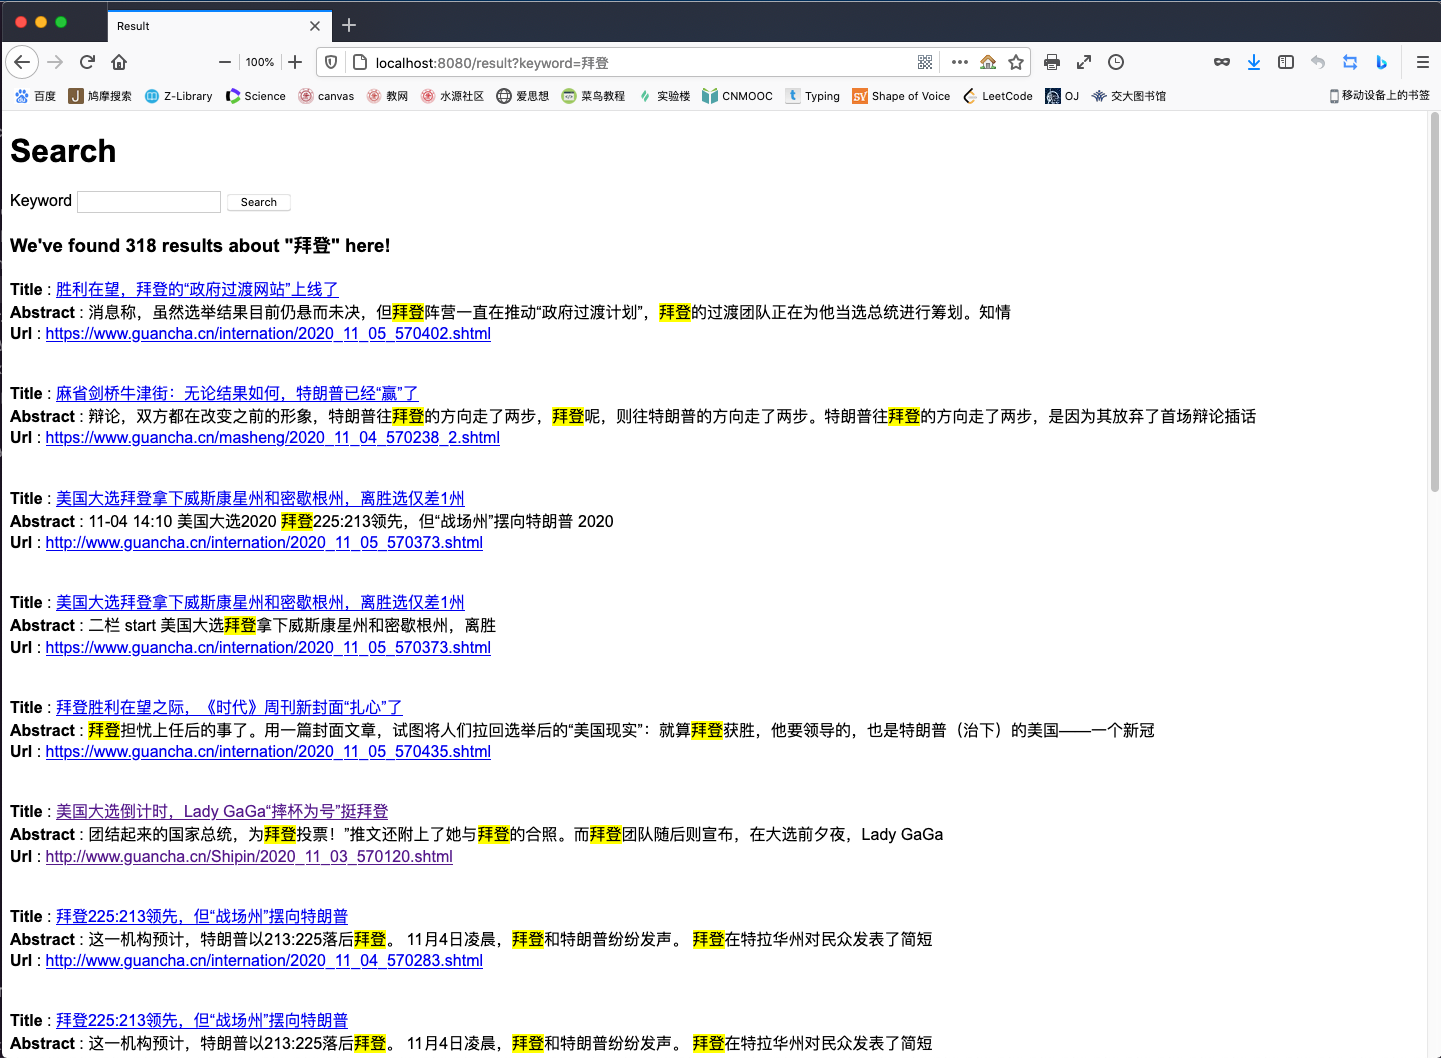
\includegraphics[scale=0.22]{img/result1.png}
            \caption{搜索页面一}
        \end{figure}

        \begin{figure}[ht]
            \centering
            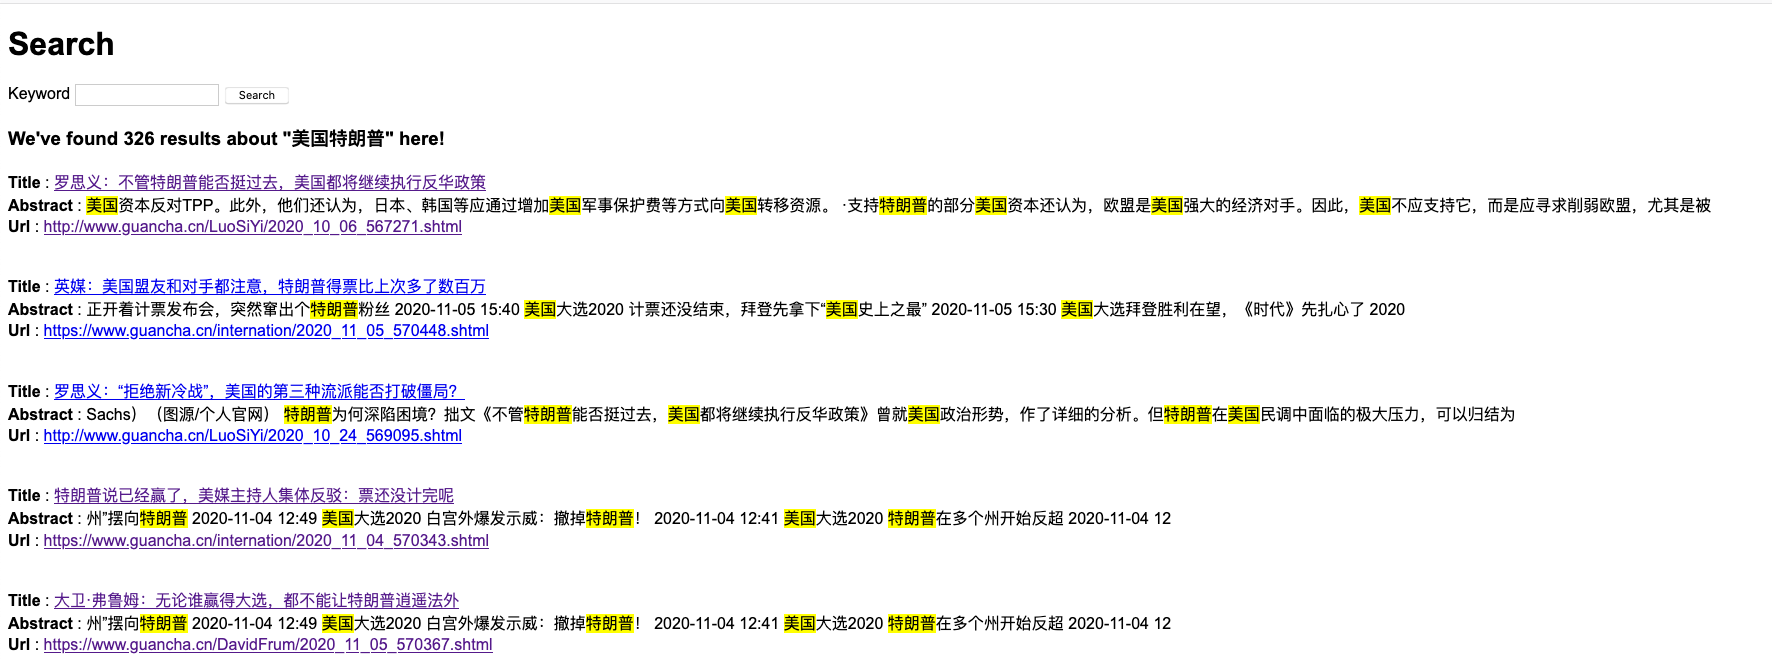
\includegraphics[scale=0.18]{img/result2.png}
            \caption{搜索页面二}
        \end{figure}


\end{document}